\chapter{Le champ électrique}
La loi de Coulomb est très utile, elle permet de calculer les caractéristiques de la force électrique. Elle pose toutefois plusieurs problèmes :
\begin{itemize}[label=\textbullet]
    \item Pour qu'une charge puisse exercer un effet sur une autre, elle doit \enquote{savoir} que celle-ci existe, mais comment le fait-elle?
    \item Si une charge est placée près d'une autre, combien de temps faut-il pour que l'effet se fasse ressentir? Rien ne peut être instantané.
\end{itemize}

Pour résoudre ces problèmes, Michael Faraday développe une idée particulièrement féconde : celle de \motcle{champ électrique}. Cette notion sera plus tard appliquée à d'autres domaine de la physique : champ de gravité, champ magnétique, champ de Higgs...


\section{Notion de champ}
Lorsqu'un radiateur est placé dans un local, il va progressivement réchauffer le local et modifier la température en chaque point de l'espace.
Lorsqu'une valeur est définie partout dans un espace ou un plan on parle de champ. Le radiateur dans le local crée ou modifie un champ de température.


\begin{figure}[!ht]
    \centering
    \begin{minipage}[b]{.47\linewidth}
        \centering
        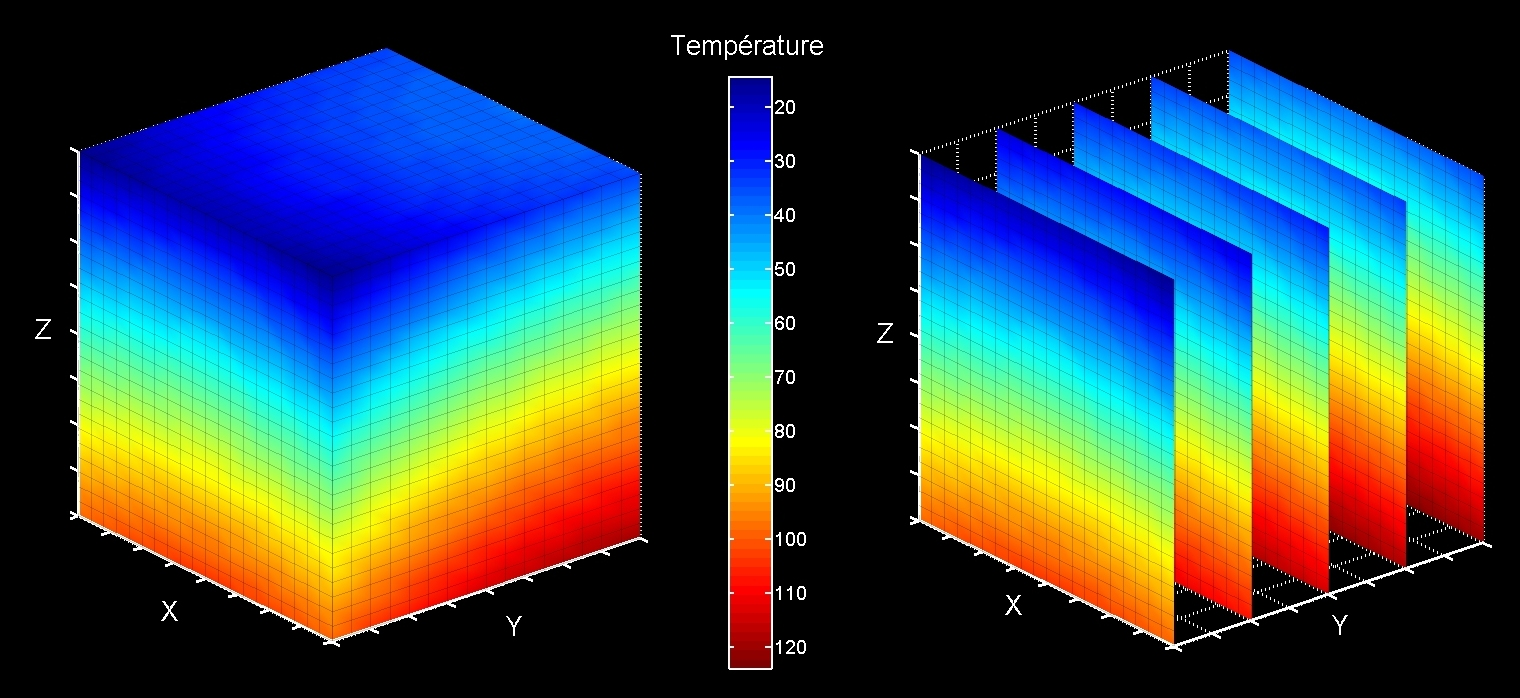
\includegraphics[width=.8\linewidth]{champ_temperature.jpg}
        \caption{Représentation d'un champ de température}
        \label{champ_temperature}
    \end{minipage}
    \begin{minipage}[b]{.47\linewidth}
        \centering
        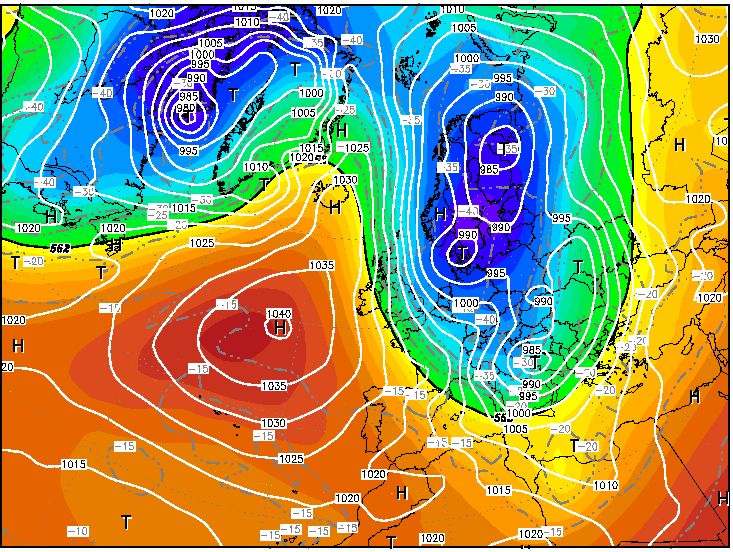
\includegraphics[width=.5\linewidth]{carte_meteo.png}
        \caption{Les cartes météo présentent souvent les champs de température et de pression.}
        \label{carte_meteo}
    \end{minipage}
\end{figure}


\newpage

\section{Champ électrique}
L'idée de Faraday est que la présence d'une charge modifie les propriétés de l'espace autour d'elle. On peut envisager qu'en tous points de l'espace il existe un champ électrique. Sa valeur peut être nulle, mais la présence de charges modifie celle-ci.
Lorsqu'une charge est placée dans un champ électrique, elle ne subit pas l'influence des autres charges mais l'influence du champ à l'endroit où elle se trouve. C'est le champ électrique qui agit sur les charges, c'est lui qui exerce la force électrique.

\begin{encadre}
    \(\vec{F_{elec}}=\vec{E} \cdot q\), où :
    \begin{itemize}[label=\textbullet]
        \item \(\vec{F_{elec}}\) est le vecteur représentant la force électrique, en \([N]\);
        \item \(\vec{E}\) est le vecteur représentant le champ électrique, en \([V \cdot m^{-1}]\) ou \([N \cdot q^{-1}]\);
        \item q est la valeur de la charge, en \([C]\).
    \end{itemize}
\end{encadre}

Par conséquent, la valeur du champ créé par une charge dans l'espace qui l'entoure vaut :
\begin{encadre}
    \(\vec{E}=\frac{1}{4 \pi \varepsilon} \frac{q}{r^2}\)
\end{encadre}

\begin{figure}[h!]
    \centering
    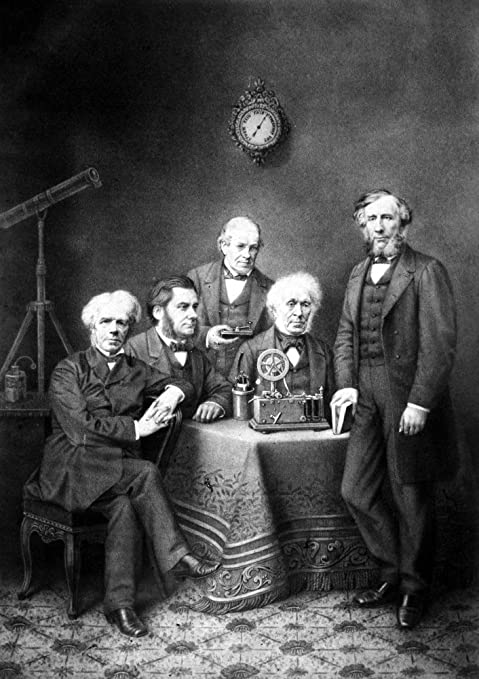
\includegraphics[width=0.35\linewidth]{faraday_and_cie.jpg}
    \caption{Michael Faraday, Thomas Henry Huxley, Charles Wheatstone, David Brewster et John Tyndall.}
    \label{club5}
\end{figure}

\newpage


\section{Sens et direction du champ}
Par convention, les vecteurs champ électrique sont toujours dirigés de manière à fuir les charges positives et à converger vers les charges négatives.
\begin{figure}[!ht]
    \centering
    \begin{minipage}[b]{.47\linewidth}
        \centering
        \resizebox{.8\linewidth}{!}{\begin{tikzpicture}
\definecolor{NavyBlue}{HTML}{7279ff}
\definecolor{DarkGreen}{HTML}{20ab2b}
\tikzset{>=latex}
\tkzInit[xstep=1 , ystep=1]
\tkzInit[xmin=-2,xmax=2,ymin=-2,ymax=2]


\tkzDefPoints{0/0/O, 1/0/A, 2/0/B, 3/0/C}

\foreach \angle in {45,90,135,180,225,270,315,360}{
\tkzDefPointBy[rotation=center O angle \angle](A)
\tkzGetPoint{Q}
\tkzDefPointBy[rotation=center O angle \angle](B)
\tkzGetPoint{R}
\tkzDrawSegment[->,color=black,thin](Q,R)}

\foreach \angle in {45,90,135,180,225,270,315,360}{
\tkzDefPointBy[rotation=center O angle \angle](C)
\tkzGetPoint{R}
\tkzDrawSegment[color=black,thin,loosely dashed](O,R)}

\tkzDrawPoint[shading=ball,ball color=green,size=10,draw=none](O)
\tkzLabelPoint(O){\textbf{+q}}


\end{tikzpicture} 
}
        \caption{Direction des vecteurs champ électrique, charge positive.}
        \label{vecteur_champ_q+}
    \end{minipage}
    \begin{minipage}[b]{.47\linewidth}
        \centering
        \resizebox{.8\linewidth}{!}{\begin{tikzpicture}
\definecolor{NavyBlue}{HTML}{7279ff}
\definecolor{DarkGreen}{HTML}{20ab2b}
\tikzset{>=latex}
\tkzInit[xstep=1 , ystep=1]
\tkzInit[xmin=-2,xmax=2,ymin=-2,ymax=2]


\tkzDefPoints{0/0/O, 1/0/A, 2/0/B, 3/0/C}

\foreach \angle in {45,90,135,180,225,270,315,360}{
\tkzDefPointBy[rotation=center O angle \angle](A)
\tkzGetPoint{Q}
\tkzDefPointBy[rotation=center O angle \angle](B)
\tkzGetPoint{R}
\tkzDrawSegment[->,color=black,thin](R,Q)}

\foreach \angle in {45,90,135,180,225,270,315,360}{
\tkzDefPointBy[rotation=center O angle \angle](C)
\tkzGetPoint{R}
\tkzDrawSegment[color=black,thin,loosely dashed](O,R)}

\tkzDrawPoint[shading=ball,ball color=red,size=10,draw=none](O)
\tkzLabelPoint(O){\textbf{-q}}



\end{tikzpicture} 
}
        \caption{Direction des vecteurs champ électrique, charge négative.}
        \label{vecteur_champ_q-}
    \end{minipage}
\end{figure}

\newpage

\section{Représentation des champs : les lignes de champ}
Il existe plusieurs possibilités pour représenter un champ:
\begin{itemize}[label=\textbullet]
    \item dessiner un ensemble de vecteurs
    \item tracer des lignes reliant les points pour lesquels le champ a la même intensité : les équipotentielles de champ.
    \item tracer des lignes qui suivent le chemin le long duquel le champ varie le plus : \motcle{les lignes de champs}. Les lignes de champs sont toujours orthogonales aux équipotentielles.
\end{itemize}
La représentation par lignes de champ permet de se faire une idée de l'aspect de celui-ci lorsque deux charges de signes opposée ou de même signe se trouvent à proximité l'une de l'autre.

\newpage

\begin{figure}[h!]
    \centering
    \resizebox{.6\linewidth}{!}{\begin{tikzpicture}
\definecolor{NavyBlue}{HTML}{7279ff}
\definecolor{DarkGreen}{HTML}{20ab2b}
\definecolor{DarkRed}{HTML}{d40004}

\tikzset{>=latex}
%\tkzInit[xstep=1 , ystep=1]
%\tkzInit[xmin=-2,xmax=2,ymin=-2,ymax=2]


\tkzDefPoints{0/0/O, 1/0/A, 2.05/0/B, 2.35/0/C, 2.55/0/D}
\tkzDefPoints{2/0/A', 2.288/0/B', 2.531/0/C', 2.704/0/D'}
\tkzDrawSegments[->,ultra thin](A,A' B,B' C,C' D,D')

\foreach \angle in {30,60,90,120,150,180,210,240,270,300,330,360}{
\tkzDefPointBy[rotation=center O angle \angle](A)
\tkzGetPoint{Q}
\tkzDefPointBy[rotation=center O angle \angle](A')
\tkzGetPoint{R}
\tkzDrawSegment[->,color=DarkRed,thin](Q,R)

\tkzDefPointBy[rotation=center O angle \angle](B)
\tkzGetPoint{Q}
\tkzDefPointBy[rotation=center O angle \angle](B')
\tkzGetPoint{R}
\tkzDrawSegment[->,color=DarkRed,thin](Q,R)

\tkzDefPointBy[rotation=center O angle \angle](C)
\tkzGetPoint{Q}
\tkzDefPointBy[rotation=center O angle \angle](C')
\tkzGetPoint{R}
\tkzDrawSegment[->,color=DarkRed,thin](Q,R)

\tkzDefPointBy[rotation=center O angle \angle](D)
\tkzGetPoint{Q}
\tkzDefPointBy[rotation=center O angle \angle](D')
\tkzGetPoint{R}
\tkzDrawSegment[->,color=DarkRed,thin](Q,R)

}


\tkzDrawPoint[shading=ball,ball color=green,size=10,draw=none](O)
\tkzLabelPoint(O){\textbf{+q}}



\end{tikzpicture} 
}
    \caption{Représentation du champ par plusieurs vecteurs.}
    \label{vecteurs_champ}
\end{figure}

\begin{figure}[h!]
    \centering
    \resizebox{.6\linewidth}{!}{\begin{tikzpicture}
\definecolor{NavyBlue}{HTML}{7279ff}
\definecolor{DarkGreen}{HTML}{20ab2b}
\definecolor{steelblue31119180}{RGB}{31,119,180}
\definecolor{orangered255440}{RGB}{255,44,0}
\definecolor{darkred17000}{RGB}{170,0,0}
\tikzset{>=latex}
\tkzInit[xstep=1 , ystep=1]
\tkzInit[xmin=-5,xmax=5,ymin=-5,ymax=5]


\tkzDefPoints{0/0/O, 1/0/A, 2/0/B, 3/0/C, 4/0/D, 4.5/0/E, 5/0/F}

\tkzDrawCircles[color=darkred17000,thin](O,A O,B O,C O,D)

\foreach \angle in {60,120,180,240,300,360}{
\tkzDefPointBy[rotation=center O angle \angle](E)
\tkzGetPoint{R}
\tkzDrawSegments[->,color=orangered255440,thin](O,R)}

\foreach \angle in {60,120,180,240,300,360}{
\tkzDefPointBy[rotation=center O angle \angle](F)
\tkzGetPoint{R}
\tkzDrawSegments[color=steelblue31119180,thin](O,R)}

\tkzDrawPoint[shading=ball,ball color=green,size=10,draw=none](O)
\tkzLabelPoint(O){+q}


\end{tikzpicture} 
}
    \caption{Représentation du champ par équipotentielles (en bleu) et lignes de champ (en rouge).}
    \label{equipotentielle}
\end{figure}

\newpage

\begin{figure}[!ht]
    \centering
    \begin{minipage}[b]{.4\linewidth}
        \centering
        \resizebox{.9\linewidth}{!}{\input{./tikz/champ_pos_neg.pstricks}}
        \caption{Lignes de champ (en rouge) et équipotentielles (en bleu) entre deux charges de signes opposés.}
        \label{champ_pos_neg}
    \end{minipage}
    \begin{minipage}[b]{.4\linewidth}
        \centering
        \resizebox{.9\linewidth}{!}{\input{./tikz/champ_pos_pos.pstricks}}
        \caption{Lignes de champ (en rouge) et équipotentielles (en bleu) entre deux charges de mêmes signes.}
        \label{champ_pos_pos}
    \end{minipage}
\end{figure}



\begin{figure}[!ht]
    \centering
    \resizebox{.7\linewidth}{!}{\input{./tikz/six_charges.pstricks}}
    \caption{Lignes de champ et équipotentielles entre six charges positives entourant une charge négative.}
    \label{six_charges}
\end{figure}


\newpage

\section{Exercices}
\begin{exercise}
    Détermine la grandeur et la direction du champ électrique en un point situé directement au-dessus d'une charge de \(50 \times 10^{-5}[C]\) et à \(35[cm]\) de celle-ci.
\end{exercise}

\begin{exercise}
    La force électrique s'exerçant sur sur une charge de \(+2 [\mu C]\) correspond à \(F=8 \times 10{-4}[N]\). Calcule la valeur du champ électrique à l'endroit de cette charge.
\end{exercise}

\begin{exercise}
    Un proton (\(m=6,67 \times 10^{-27}[kg]\)) immobile se trouve en suspension dans le champ gravitationnel à proximité de la surface terrestre et dans un champ électrique uniforme \(\vec{E}\). Détermine les caractéristiques de \(\vec{E}\).
\end{exercise}

\begin{exercise}
    Détermine les caractéristiques du champ électrique en un coin d'un carré de \(80[cm]\) de côté s'il y a des charges \(18,2 \times 10^{-7}[C]\) aux trois autres coins.
\end{exercise}

\begin{exercise}
    Détermine les caractéristiques du champ électrique au sommet d'un triangle équilatéral de \(10[cm]\) de côté si les deux autres sommets sont occupés par une charge de \(6 \times 10^{-7}[C]\)
\end{exercise}

\begin{figure}[h!]
    \centering
    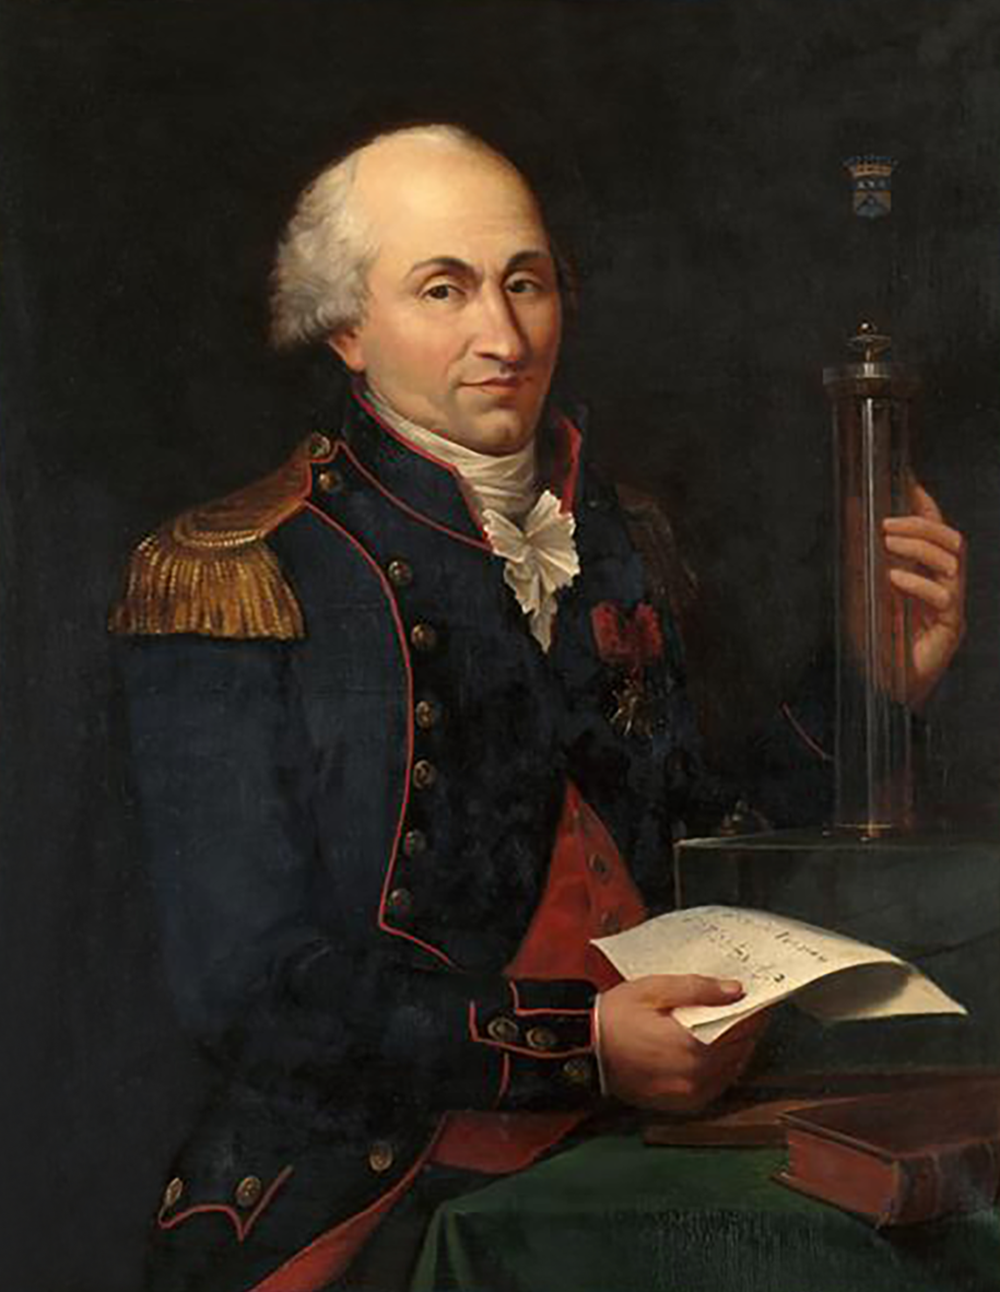
\includegraphics[width=0.4\linewidth]{charles_coulomb.png}
    \caption{Charles-Augustin Coulomb(1736 - 1806).}
    \label{charles_coulomb}
\end{figure}
